\documentclass[notes,11pt, aspectratio=169]{beamer}

\usepackage{pgfpages}
% These slides also contain speaker notes. You can print just the slides,
% just the notes, or both, depending on the setting below. Comment out the want
% you want.
\setbeameroption{hide notes} % Only slide
%\setbeameroption{show only notes} % Only notes
%\setbeameroption{show notes on second screen=right} % Both

\usepackage{helvet}
\usepackage[default]{lato}
\usepackage{array}

\usepackage{caption}
\usepackage{subcaption}

\usepackage{tikz}
\usepackage{verbatim}
\setbeamertemplate{note page}{\pagecolor{yellow!5}\insertnote}
\usetikzlibrary{positioning}
\usetikzlibrary{calc}
\usetikzlibrary{arrows}
\usetikzlibrary{decorations.markings}
\usetikzlibrary{shapes.misc}
\usetikzlibrary{matrix,shapes,arrows,fit,tikzmark}
\usepackage{amsmath}
\usepackage{mathpazo}
\usepackage{lipsum}
\usepackage{amsmath, amsfonts, amssymb}
\usepackage{multimedia}
\usepackage{graphicx}
\usepackage{multirow}
\usepackage{graphicx}
\usepackage{dcolumn}
\usepackage{bbm}
\newcolumntype{d}[0]{D{.}{.}{5}}

\usepackage{changepage}
\usepackage{appendixnumberbeamer}
\newcommand{\beginbackup}{
   \newcounter{framenumbervorappendix}
   \setcounter{framenumbervorappendix}{\value{framenumber}}
   \setbeamertemplate{footline}
   {
     \leavevmode%
     \hline
     box{%
       \begin{beamercolorbox}[wd=\paperwidth,ht=2.25ex,dp=1ex,right]{footlinecolor}%
%         \insertframenumber  \hspace*{2ex} 
       \end{beamercolorbox}}%
     \vskip0pt%
   }
 }
\newcommand{\backupend}{
   \addtocounter{framenumbervorappendix}{-\value{framenumber}}
   \addtocounter{framenumber}{\value{framenumbervorappendix}} 
}


\usepackage{graphicx}
\usepackage[space]{grffile}
\usepackage{booktabs}

\DeclareUnicodeCharacter{0301}{\'{e}}
\DeclareUnicodeCharacter{0303}{}

% These are my colors -- there are many like them, but these ones are mine.
\definecolor{blue}{RGB}{0,114,178}
\definecolor{red}{RGB}{213,94,0}
\definecolor{yellow}{RGB}{240,228,66}
\definecolor{green}{RGB}{0,158,115}




%% I use a beige off white for my background
\definecolor{MyBackground}{RGB}{255,253,218}

%% Uncomment this if you want to change the background color to something else
%\setbeamercolor{background canvas}{bg=MyBackground}

%% Change the bg color to adjust your transition slide background color!
\newenvironment{transitionframe}{
  \setbeamercolor{background canvas}{bg=yellow}
  \begin{frame}}{
    \end{frame}
}

\setbeamercolor{frametitle}{fg=blue}
\setbeamercolor{title}{fg=black}
\setbeamertemplate{footline}[frame number]
\setbeamertemplate{navigation symbols}{} 
\setbeamertemplate{itemize items}{-}
\setbeamercolor{itemize item}{fg=blue}
\setbeamercolor{itemize subitem}{fg=blue}
\setbeamercolor{enumerate item}{fg=blue}
\setbeamercolor{enumerate subitem}{fg=blue}
\setbeamercolor{button}{bg=MyBackground,fg=blue,}



% If you like road maps, rather than having clutter at the top, have a roadmap show up at the end of each section 
% (and after your introduction)
% Uncomment this is if you want the roadmap!
 \AtBeginSection[]
 {
    \begin{frame}
        \frametitle{Roadmap of Talk}
        \tableofcontents[currentsection]
    \end{frame}
 }
\setbeamercolor{section in toc}{fg=blue}
\setbeamercolor{subsection in toc}{fg=red}
\setbeamersize{text margin left=30pt,text margin right=30pt} 

\newenvironment{wideitemize}{\itemize\addtolength{\itemsep}{10pt}}{\enditemize}

\usepackage{environ}
\NewEnviron{videoframe}[1]{
  \begin{frame}
    \vspace{-8pt}
    \begin{columns}[onlytextwidth, T] % align columns
      \begin{column}{.58\textwidth}
        \begin{minipage}[t][\textheight][t]
          {\dimexpr\textwidth}
          \vspace{8pt}
          \hspace{4pt} {\Large \sc \textcolor{blue}{#1}}
          \vspace{8pt}
          
          \BODY
        \end{minipage}
      \end{column}%
      \hfill%
      \begin{column}{.42\textwidth}
        \colorbox{green!20}{\begin{minipage}[t][1.2\textheight][t]
            {\dimexpr\textwidth}
            Face goes here
          \end{minipage}}
      \end{column}%
    \end{columns}
  \end{frame}
}

\title[]{\textcolor{blue}{Causal Inference with Synthetic Controls}}
%\author[PGP]{}
\institute[GSB]{\small{\begin{tabular}{c}
Alexander J. Almeida \\
Stanford Graduate School of Business\\
\end{tabular}}}

\date{July 20, 2023}

\usepackage[backend=biber,style=apa]{biblatex}
\addbibresource{ref.bib}

%\usepackage{hyperref}
\hypersetup{
  colorlinks=false,
  linkcolor=, 
  urlcolor=
}


\makeatletter
\newcommand\disablecolorlinks{\def\HyColor@UseColor##1{}}
\makeatletter
\addtobeamertemplate{headline}{\disablecolorlinks{}}{}

\begin{document}

%%% TIKZ STUFF
\tikzset{   
        every picture/.style={remember picture,baseline},
        every node/.style={anchor=base,align=center,outer sep=1.5pt},
        every path/.style={thick},
        }
\newcommand\marktopleft[1]{%
    \tikz[overlay,remember picture] 
        \node (marker-#1-a) at (-.3em,.3em) {};%
}
\newcommand\markbottomright[2]{%
    \tikz[overlay,remember picture] 
        \node (marker-#1-b) at (0em,0em) {};%
}
\tikzstyle{every picture}+=[remember picture] 
\tikzstyle{mybox} =[draw=black, very thick, rectangle, inner sep=10pt, inner ysep=20pt]
\tikzstyle{fancytitle} =[draw=black,fill=red, text=white]
%%%% END TIKZ STUFF

% Title Slide
\begin{frame}
\maketitle
\end{frame}

\section{Synthetic control design: basics}

% Section 1: What is SC?
\begin{frame}{}
    % Notes
    %   1. Point out basque country and note state structure of the country.
    \begin{figure}
        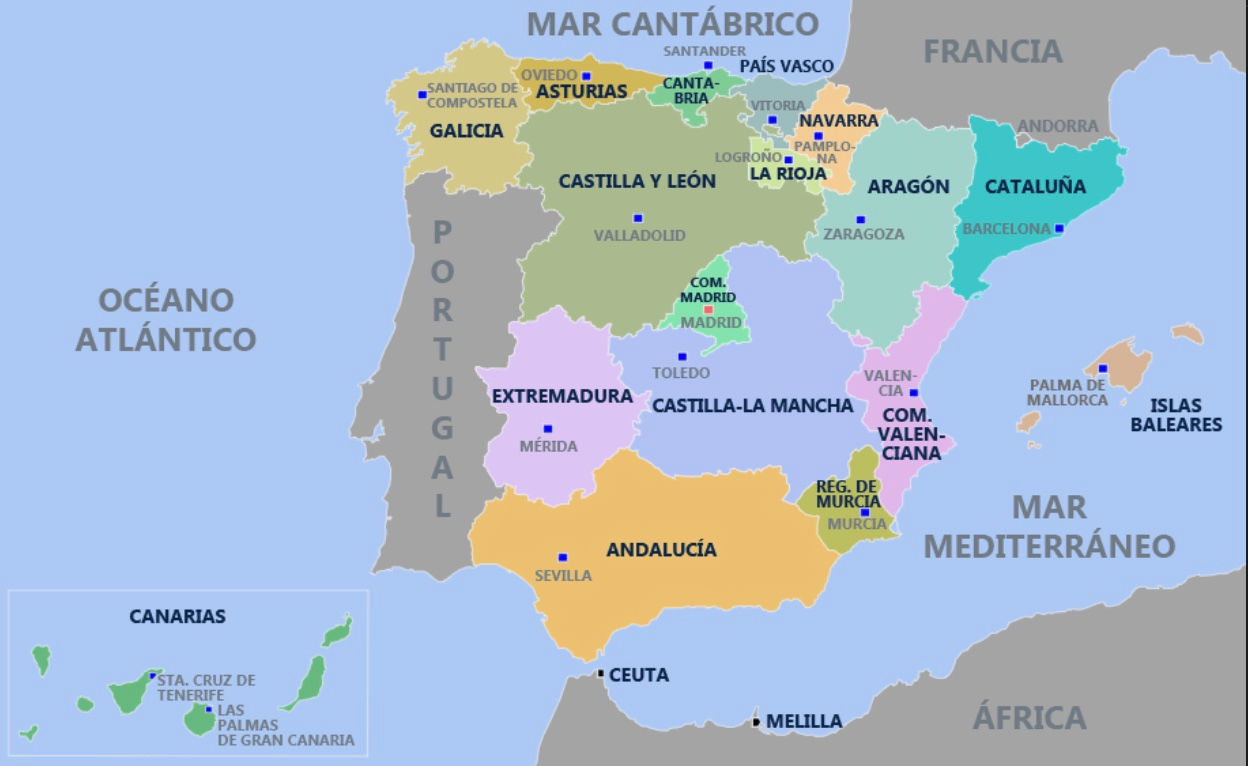
\includegraphics[width = .7\linewidth]{figures/mapa.png}
    \end{figure}
\end{frame}

\begin{frame}{}
    \begin{wideitemize}
        \item Euskadi Ta Askatasuna (ETA) formed to support Basque separatism
        \item Beginning terrorist activities in the late 1960s
    \end{wideitemize}
\end{frame}

\begin{frame}{}
    % Highlight that the killings begin in the 1960s and intensify
    %   into the 1980s. Notice that many potential confounders in this
    %   time span would make problematic a simple before and after comparison.
    \begin{figure}
        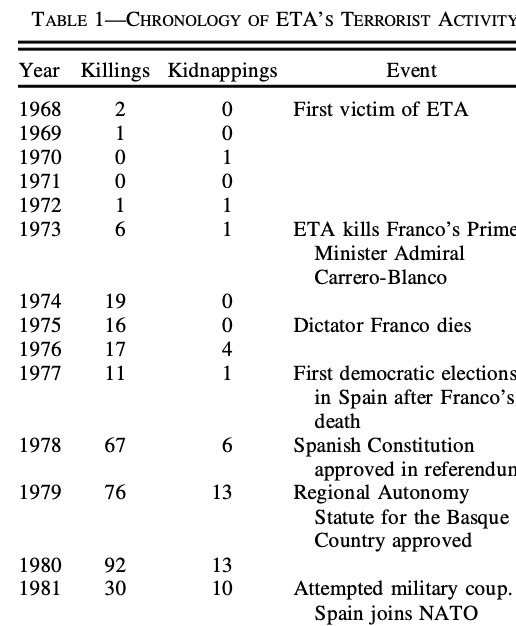
\includegraphics[width = .4\linewidth]{figures/tab11.png}
    \end{figure}
\end{frame}

\begin{frame}{}
    % Note that the end of the analysis period is 1998, although as of
    %   2017 the group is no longer active.
    \begin{figure}
        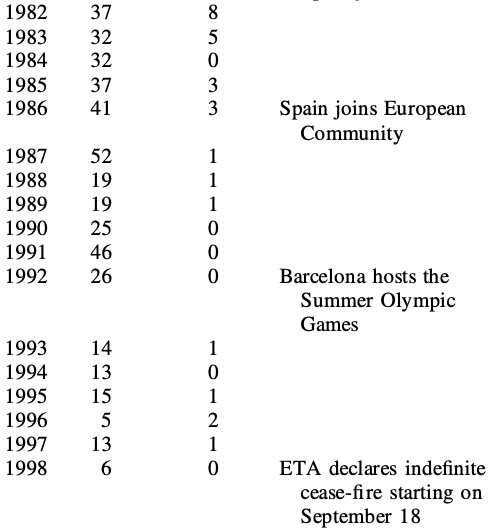
\includegraphics[width = .4\linewidth]{figures/tab12.png}
    \end{figure}
\end{frame}

\begin{frame}{}
    \begin{wideitemize}
        \item Question: What was the impact of terrorism on the people of the Basque Region? \pause 
        \item Less ambitious
        \begin{wideitemize} 
            \item What was the \textbf{economic} impact of terrorism on the people of the Basque Region? 
            \item Can we quantify this effect?
        \end{wideitemize}
    \end{wideitemize}
\end{frame}

\begin{frame}{}
    \medskip
    \begin{figure}
    \centering
        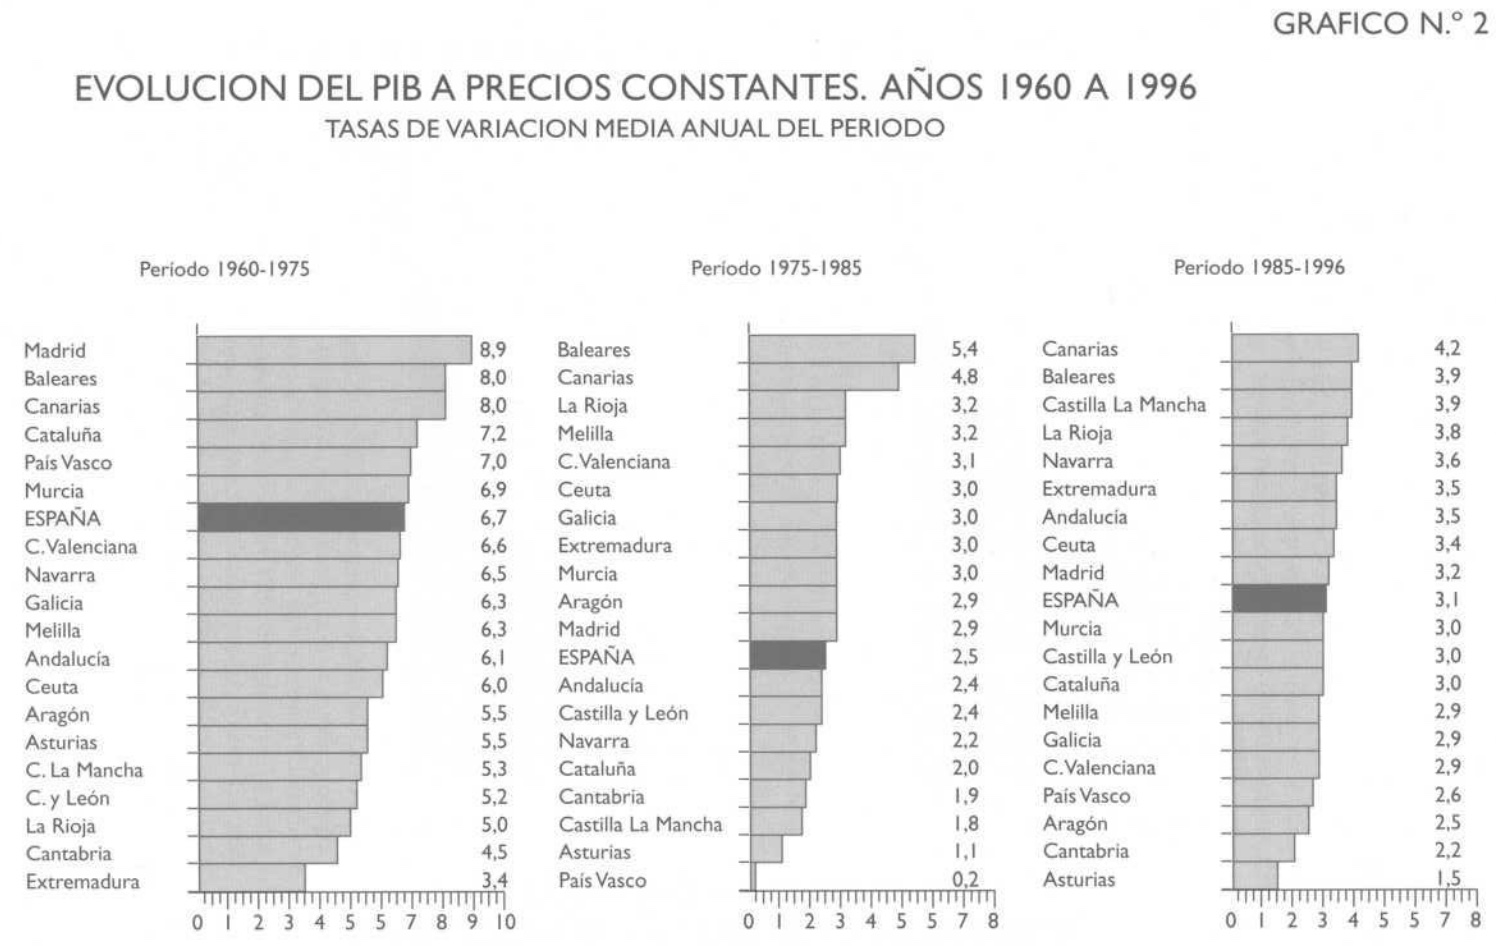
\includegraphics[width = .75\linewidth]{figures/evolucion_pib.png}
        \label{fig:evolucion}
        \caption*{\small Source: \cite{fundacion_bbv_renta_1999}}
    \end{figure}
\end{frame}

\begin{frame}{}
    How do we quantify the effect of terrorism? \pause \bigskip
    \begin{wideitemize}
        \item A na\"ive comparison of means before and after terrorism \medskip 
        \begin{wideitemize} 
            \item ignores time-varying dynamics that are independent of terrorism 
            \item e.g. Business cycle variations in macroeconomic aggregates
        \end{wideitemize}
        \item Comparing Basque country to other regions of Spain \medskip \pause
            \begin{wideitemize}
                \item Concentration of terrorism in Basque country supports this method
            \end{wideitemize}
    \end{wideitemize}    
\end{frame}

\begin{frame}{}
    How do we quantify the effect of terrorism? \pause \\
    \bigskip 
    
    \rightline{Compare the outcomes of Basque country to other regions that are similar.}
    \rightline{\textcolor{purple}{Issue: we can't just compare it to the rest of Spain.}}   
\end{frame}

\begin{frame}{}
    \begin{figure}
        \centering
        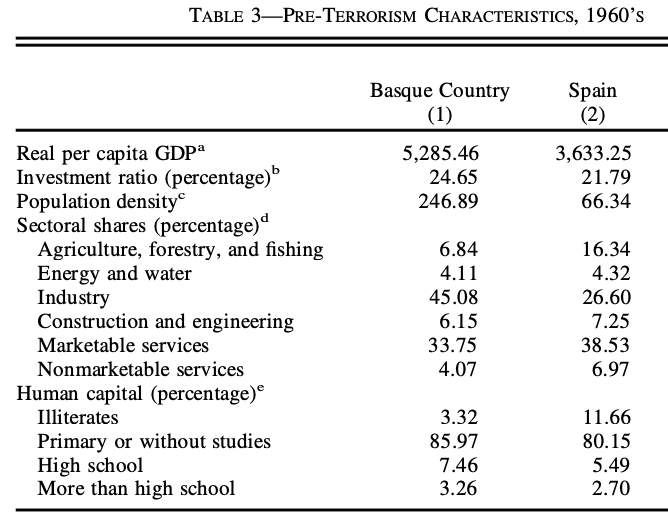
\includegraphics[width = .6\textwidth]{figures/balance panel.png}
        \label{fig:balance}
    \end{figure}
\end{frame}

\begin{frame}{}
    How do we quantify the effect of terrorism? \\
    \bigskip 
    
    \rightline{Compare the outcomes of Basque country to other regions that \textbf{are similar}.} \pause 

    \bigskip \bigskip 
    
    Any experimental control group of this form will be a weighted average of the options available. \medskip
        \begin{wideitemize}
           \item A difference in difference (DID) strategy would weight non-basque autonomous communities equally
           \item We can choose the weights more carefully: \textbf{synthetic control}
        \end{wideitemize}

    \medskip

    The synthetic control method as we currently know it is developed in 
    \cite{abadie_economic_2003}.
    
\end{frame}

\begin{frame}{Empirical considerations}
    \begin{figure}
        \centering
        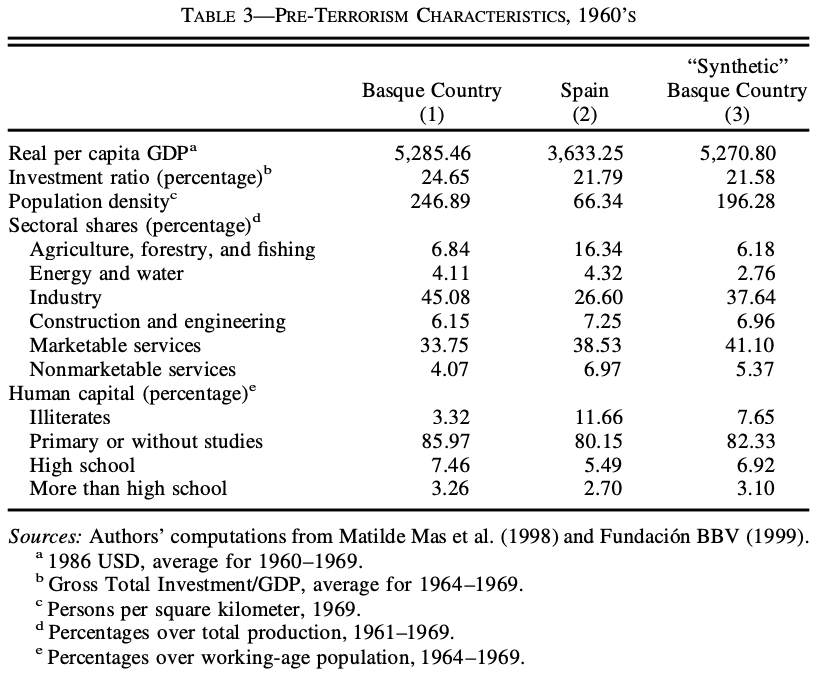
\includegraphics[width = .6\textwidth]{figures/balance panel all.png}
        \label{fig:balance_all-2}
    \end{figure}
\end{frame}

\begin{frame}{}
    \begin{wideitemize}
        \item Suppose there are $J$ potential control regions. \pause 
        \item Let $W = (w_1, \ldots, w_J)' \in \mathbb R^J$ be the weights. Each $W$ corresponds to 
        a different synthetic control region. Usually we will want nonnegative 
        weights that sum to 1.\pause 
        \item Goal: Choose $W$ such that the synthetic control region resembles the actual region. \pause \medskip
        \begin{wideitemize}
            \item Let $X_1 \in \mathbb R^K$ be the vector of pre-treatment observables. 
            \item Let $X_0 \in \mathbb R^{K \times J}$ be the matrix of pre-treatment observables for all regions. 
            \item We want to minimize $\| X_1 - X_0 W\|$
        \end{wideitemize}
    \end{wideitemize}
\end{frame}

\begin{frame}{}
    \begin{itemize}
        \item We could minimize using the Euclidian norm
        \[ \| X_1 - X_0 W \| = \sqrt{\sum _{k=1}^K \left(X_1^k - X_0^k W\right) ^ 2 },\]
        but we can incorporate greater flexibility by weighting the $k$th covariate
        by a value $V_{kk} \in \mathbb R$. \pause
        \item Operationalize this by letting $V \in \mathbb R^{K \times K}$ be 
        diagonal (thus defining a semi-norm, see \cite{abadie_synthetic_2010}) 
        where we collect the weights $V_{kk}$ along the diagonal. 
        \[\|X_1 - X_0 W\|_V := (X_1 - X_0 W)' V (X_1 - X_0W)\] \pause  
        \item What should we choose for $V$? 
    \end{itemize}
\end{frame}

\begin{frame}{}
        The weighting matrix $V$ could be chosen to weight relative importance of matching
        specific predictors (think 2-step GMM).
        
        \medskip
       
        Instead, we will choose the matrix $V$ to match the treated unit's time series in
        the outcome variable.
        
    \bigskip

    Algorithm:\pause
    \begin{itemize}
    
            \item Let $\mathcal W$ denote the set of nonnegative weights in $\mathbb R^K$ that sum
            to one. For each weighting matrix $V$, 
            choose weights to minimize the weighted sum of squared errors, 
            \[ W^*(V) = \text{argmin}_{W \in \mathcal W} (X_1 - X_0 W)' V (X_1 - X_0 W) \] \pause 
            \item For each balanced synthetic control $W^*(V)$, choose $V$ to minimize the difference
            between the time series of the treated unit and the synthetic control.
            
    \end{itemize}    
    
\end{frame}

\begin{frame}{}
    Performing this method tells us that 
    \[\texttt{Basque} = 0.8508(\texttt{Catalonia}) + 0.1492 (\texttt{Madrid})\]

    \pause Based on the construction, we expect that  \medskip 
    \begin{wideitemize}
        \item pre-intervention observables of Basque region and synthetic Basque region are close, and
        \item pre-intervention per capita GDP time series for Basque and synthetic Basque regiones are close
    \end{wideitemize}
\end{frame}


\begin{frame}{}
    \begin{figure}
        \centering
        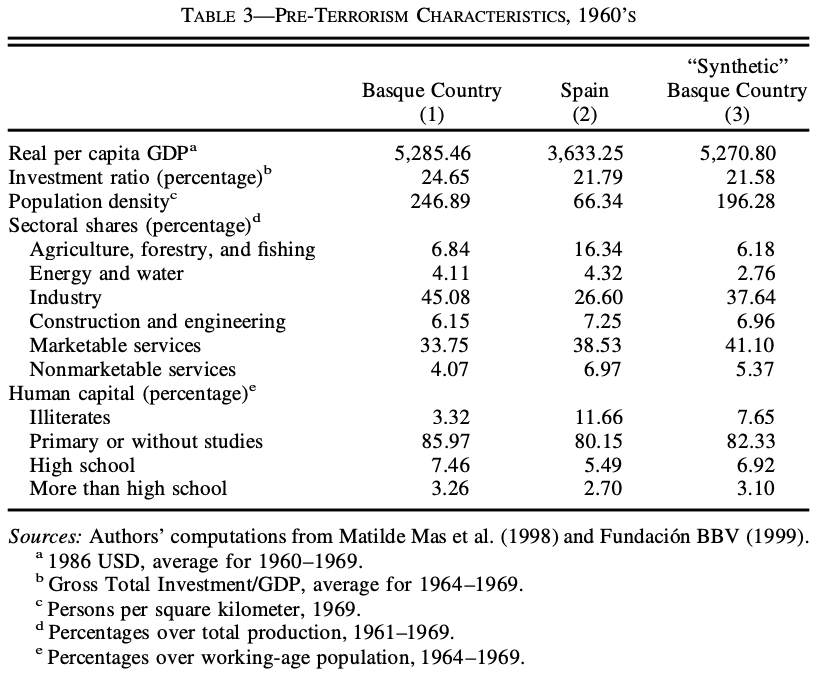
\includegraphics[width = .6\textwidth]{figures/balance panel all.png}
        \label{fig:balance_all}
    \end{figure}
\end{frame}

\begin{frame}{}
    \begin{figure}
        \centering
        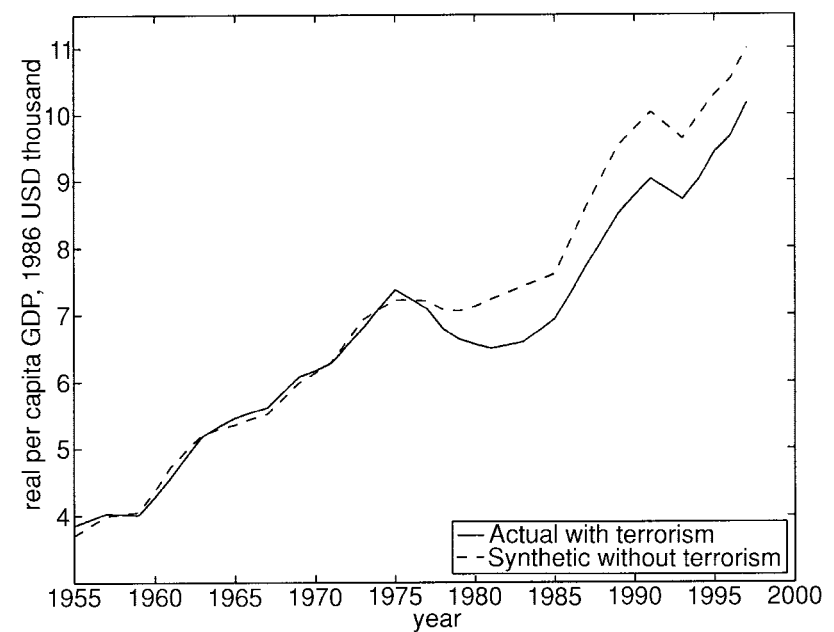
\includegraphics[width = .6\textwidth]{figures/ts.png}
        \label{fig:ts}
    \end{figure}
\end{frame}

\begin{frame}

    \begin{wideitemize}
        \item No formal ``inferences" are made in the paper: confidence
        bounds, standard errors
        \item Instead, the authors conduct a falsification exercise.
        
        \medskip 
        
        \begin{wideitemize}
            \item Suppose that in fact Catalonia experienced terrorism, and
            not the Basque Country.
            \item If we conduct the same analysis on Catalonia and find
            a discrepancy between the synthetic Catalonia and the real
            Catalonia then we are in trouble.
        \end{wideitemize}
    \end{wideitemize}
    
\end{frame}


\begin{frame}{}
    \begin{figure}
        \centering
        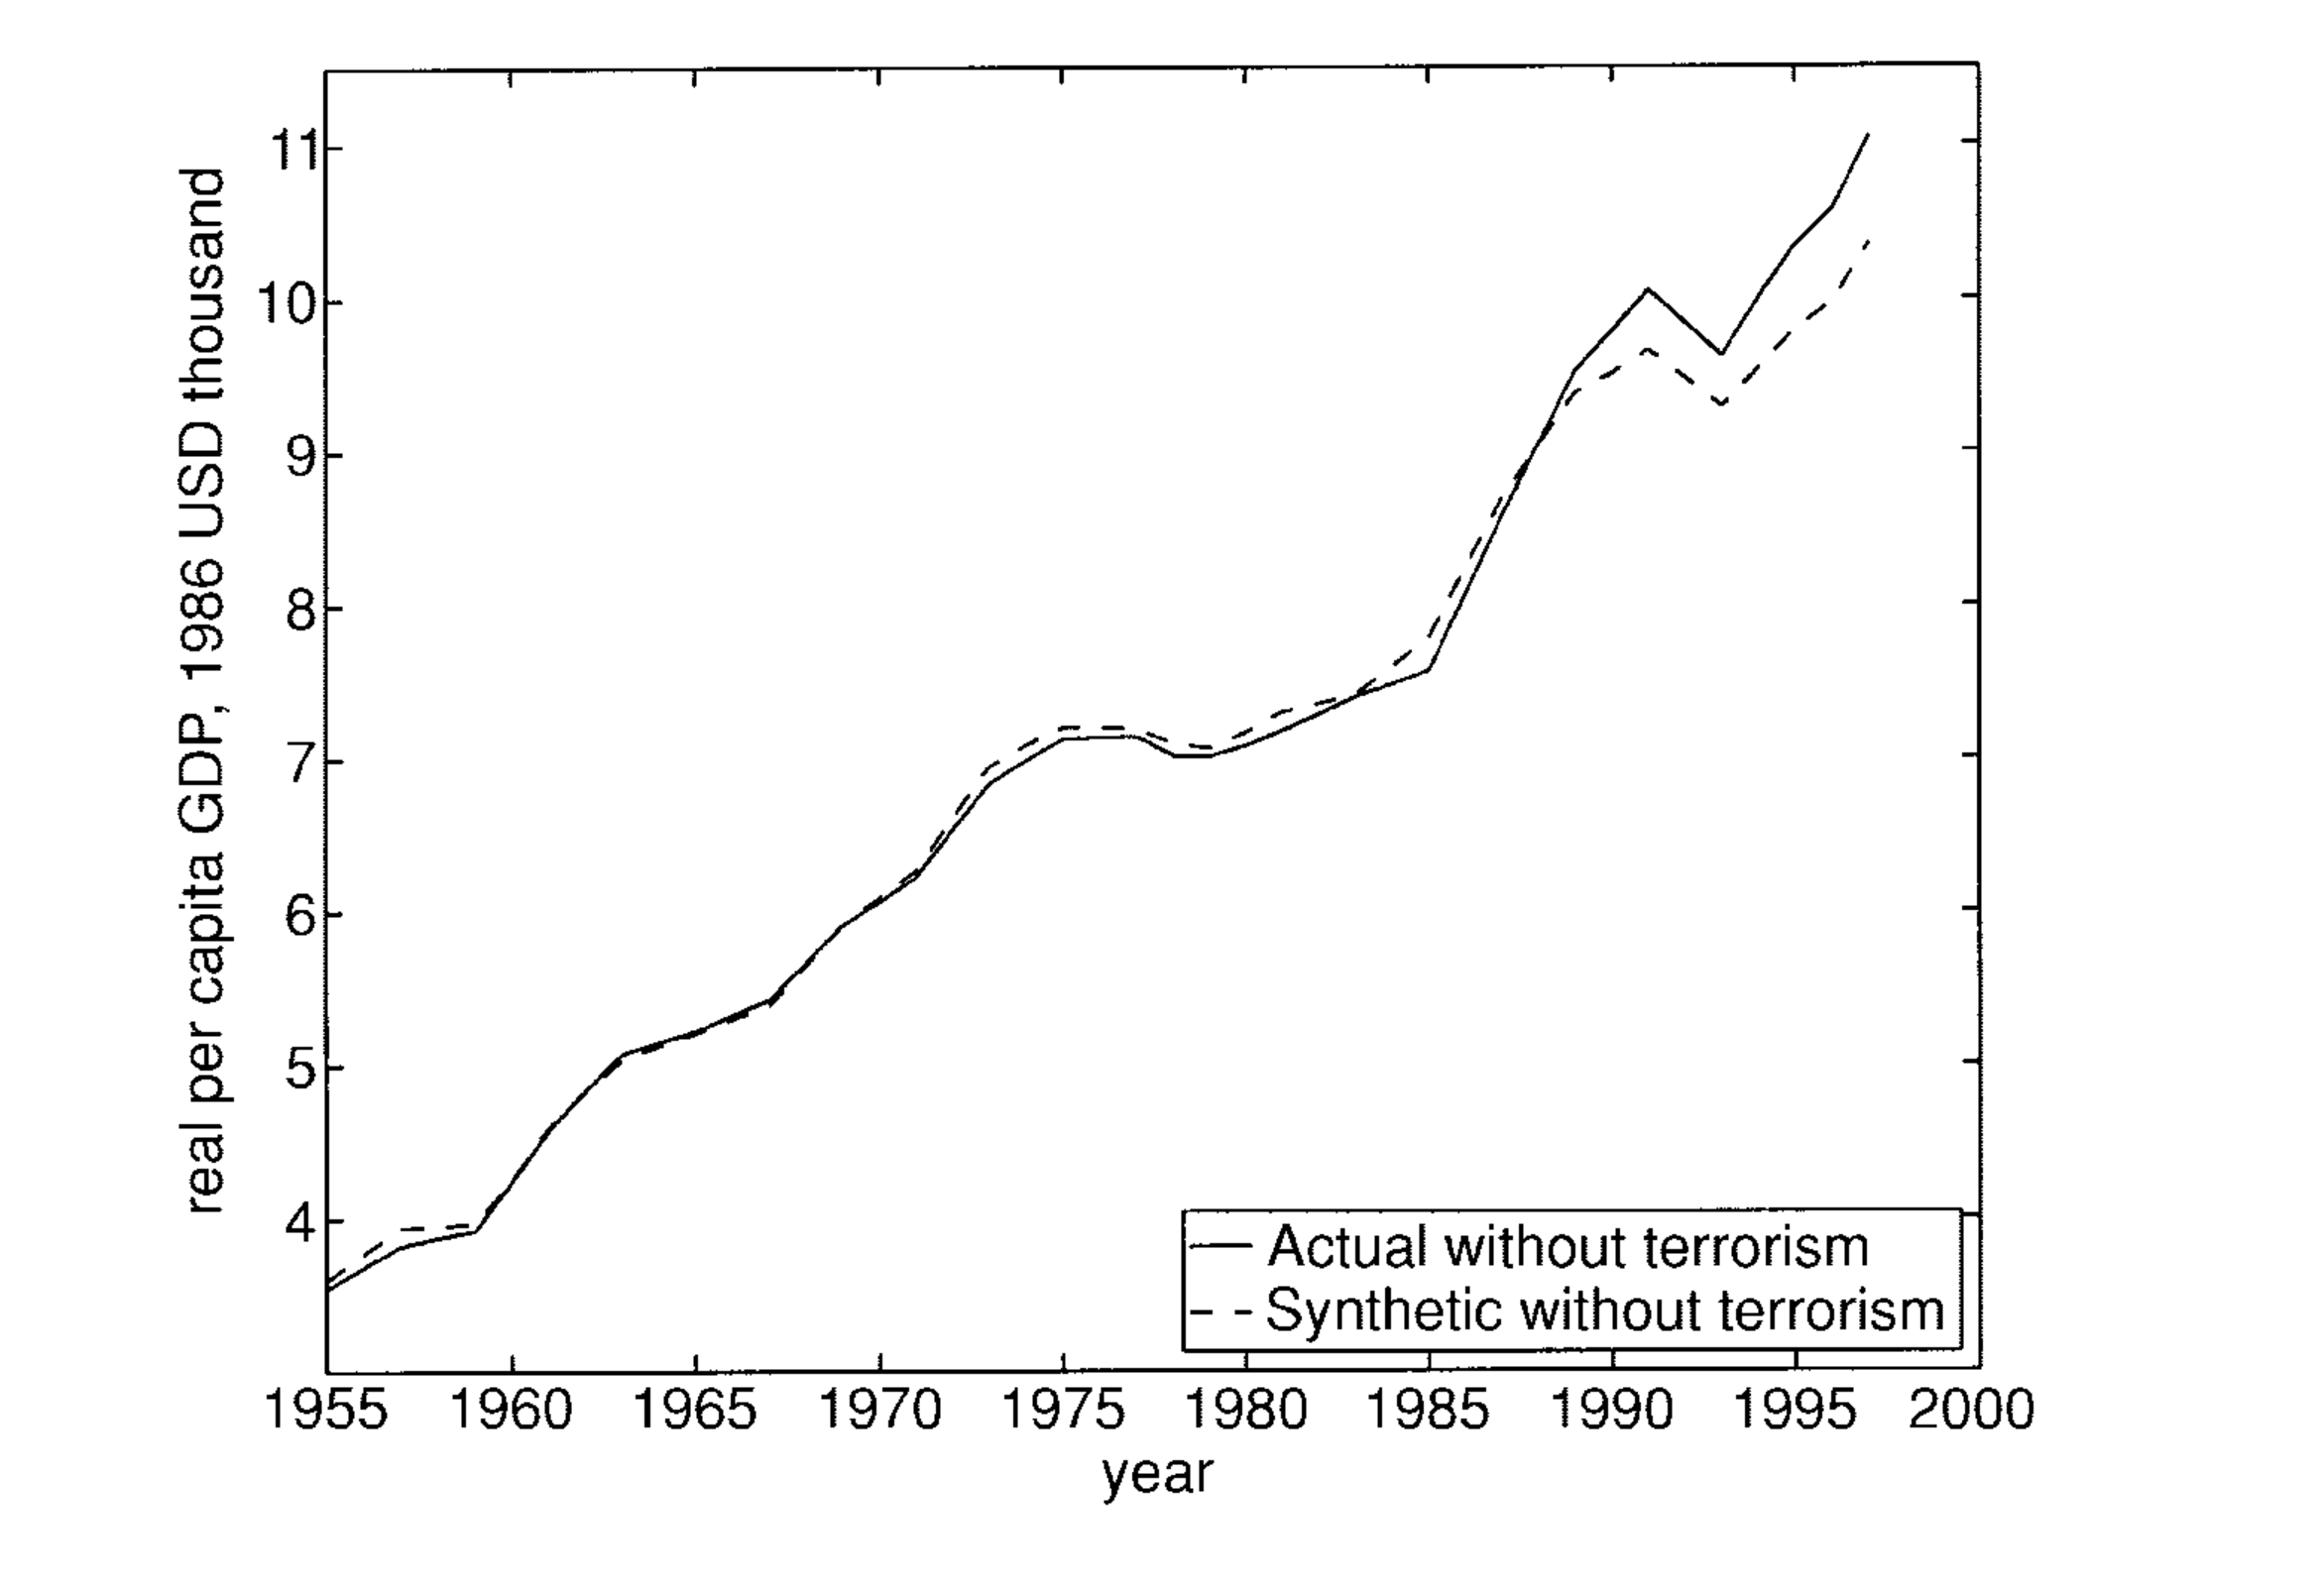
\includegraphics[width = .7 \linewidth]{figures/ag2003_cat.png}
        \caption*{ \tiny The results of conducting a ``placebo test" using the data from 
        \cite{abadie_economic_2003}. A synthetic control is built for Catalonia, with
        the Basque Country excluded from the donor pool. Notice that the resulting time
        series reproduces the actual time series precisely until the late 1980s. Also relevant is the fact that the olympics took place in Barcelona in 1992.}
        \label{fig:enter-label}
    \end{figure}
\end{frame}

\begin{frame}{}

    \begin{wideitemize}
        \item Outstanding question: is the result significant?
        \item The authors spend time offering arguments that it is, but we don't have
            any formal statistical model at this point.
        \item Subsequent papers make strides in this direction leveraging
            randomization inference framework.
    \end{wideitemize}
 
\end{frame}

\section{Randomization inference: basics}

\begin{frame}{}

    \begin{wideitemize}
        \item The idea of randomization inference is often attributed 
        to Ronald Fisher who introduced the method as an aside in his 
        textbook \textit{The Design of Experiments}
        (\cite{fisher_design_1974}).
        \item In fact, the careful formulation of the idea is better
        attributed to
        Edwin Pitman (\citeyear{pitman_significance_1937}) and
        Bernard L. Welch (\citeyear{welch_z-test_1937}).
    \end{wideitemize}
    
\end{frame}

\begin{frame}
    
        It's argued that the idea's attribution is an example of
        Stigler's law of eponymy (\cite{onghena_randomization_2017}):

        
      \begin{block}{}
        ``No scientific discovery is named after its original discoverer."
      \end{block}

      % stigler attributes the idea to Robert K. Merton, the sociologist.
    
      \begin{flushright}
        - Stephen Stigler
      \end{flushright}
      
\end{frame}

\begin{frame}
    
    Consider this example.
   
    \medskip
    
    \begin{wideitemize}
        \item Three students are given a study guide before an exam and three are not.
        \item The scores are \(x_0 = (\textcolor{green}{85}, \textcolor{green}{60}, \textcolor{green}{95}, \textcolor{blue}{55}, \textcolor{blue}{70}, \textcolor{blue}{85}),\)
        where the first three
        elements in the vector are the treated students' scores.
    \end{wideitemize}

    \bigskip
    
    The scores for the students that received the guide exceed the others by 10.
    Does the study guide work? \pause 
    
    \medskip

    Intuition: any three of these values are equally likely to be the treated units. 
    
    If we assume no treatment effect (i.e. $H_0: \tau = 0$), then 
    any permutation of the outcome vector, e.g. $(\textcolor{green}{85}, \textcolor{green}{60}, \textcolor{blue}{55}, \textcolor{green}{95}, \textcolor{blue}{70}, \textcolor{blue}{85})$, 
    equally likely to occur.
    \pause 

    \medskip 
    
    One solution: Enumerate all $6!$ permutations $x$ of $x_0$ \& calculate the statistic for each
    one. This gives an exact distribution of the statistic $T$.
    Comparing $T(x_0)$ to this distribution allows us to make inferential statements about the
    treatment effect.

\end{frame}


\begin{frame}{}

    \begin{figure}
        \centering
        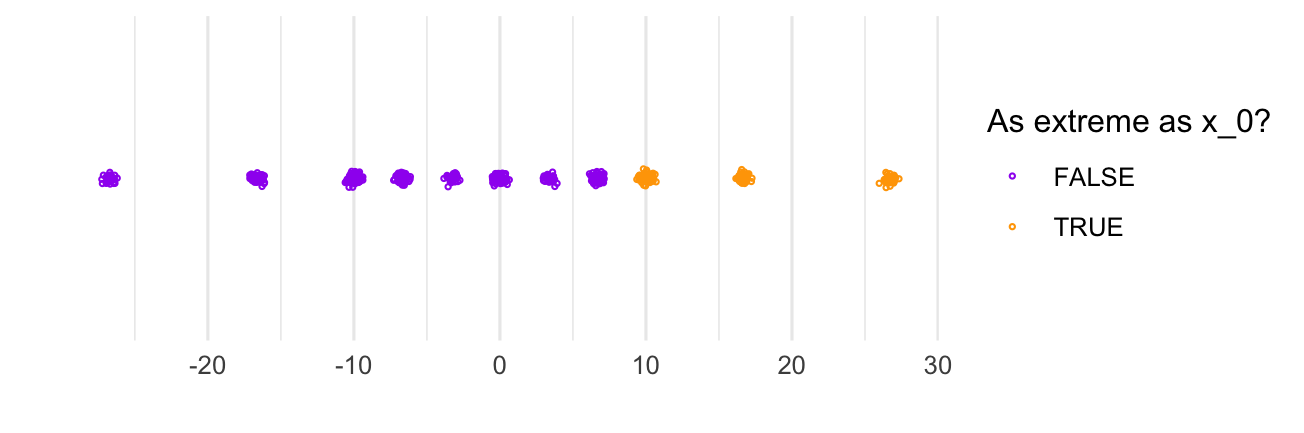
\includegraphics[width = \linewidth]{figures/rand.png}
        \caption*{\small The empirical distribution of the difference in means statistic under the assumption that all permutations of the outcome vector are equally likely. The corresponding probability of observing a result at least as surprising as 10 under the null hypothesis is 30\%.}
        \label{fig:pvalue}
    \end{figure}

\end{frame}

\begin{frame}{}

    An equivalent solution is to reason that \ldots
    \begin{itemize}
       \item The statistic $T$ depends only the partitioning of the students' scores into
       treated and untreated. 
       \item There are $\dbinom{6}{3} = 20$ ways of choosing the three treated units.
       \item  Enumerating all combinations will give us a p-value as well.
    \end{itemize}

    \medskip

    In this sense, the natural way to think about the experiment is with combinations, rather
    than permutations (see \cite{imbens_causal_2015}, Chapter 5).

\end{frame}

\begin{frame}{}

    Nomenclature for randomization inference is occasionally confusing:
    \begin{itemize}
        \item Randomization tests are occasionally called permutation tests
        \item Randomization tests are occasionally more naturally identified
            with combinations rather than permutations of the data
    \end{itemize}
    
    \bigskip 

    Worse, Onghena relates how
    the \textit{Encyclopedia of Statistical Sciences} in 1986
    published conflicting entries which simultaneously stated that:

    \begin{itemize}
        \item Randomization test is special case of permutation test (Edgington).
        \item Permutation test is special case of randomization test (Gibbons).
    \end{itemize}
    
\end{frame}


\begin{frame}{}

    Summary of randomization inference: by assuming that the treatment effect is zero we can calculate
    an exact null distribution of the statistic of interest by enumerating all of the possible assignments.

    \medskip

    We can do this for any statistic:
    \begin{itemize}
        \item Transformations of the data. Consider taking $\log$ transformations for positive data.
        \item Robust statistics: the difference in medians or the difference in mean rank are more ``robust"
        in the sense often attributed to Tukey.
        \item The $t$-statistic, but compare the statistic to the exact distribution
        rather than to the theoretical $t$-distribution.
    \end{itemize}
\end{frame}

\begin{frame}{}
A final note on randomization inference is that there is a close connection between
randomization inference and bootstrapping.

\medskip
\begin{wideitemize}
    \item Bootstrapping consists of sampling with replacement from the data.
    \item Randomization consists of sampling without replacement from the data.
\end{wideitemize}

\begin{block}{}
    ``The bootstrap distribution was originally called the `combination distribution.' It was designed to extend the virtues of permutation testing to the
    great majority of statistical problems where there is nothing to permute."
\end{block}
\begin{flushright}
    - Bradley Efron and Robert Tibshirani (\citeyear{efron_introduction_1993}, pp. 218).
\end{flushright}

\end{frame}



\section{Randomization inference for synthetic controls}

\begin{frame}{}

        Consider once again the synthetic controls set up in light of our randomization inference framework:
        \pause
        \medskip
        
        \begin{itemize}
            \item We want to compare the treated units to their synthetic controls via some statistic \pause
            \item Each placebo test calculates the same statistic (as in \cite{abadie_economic_2003}) \pause
            \item We care to determine if there is a significant effect associated with some intervention \pause
        \end{itemize}
    
        \medskip
    
        Without making any distributional assumptions about the statistic in question, we are able to
        calculate exact p-values using this methodology. This was noticed in \cite{abadie_synthetic_2010}.
    
\end{frame}

\begin{frame}{}

    \begin{wideitemize}
        \item In 1988, California voters passed \textbf{1988 Proposition 99}
        \item The law included a 25-cent excise tax per carton of cigarettes
        \item What is an appropriate counterfactual? \pause \textcolor{red}{\textbf{Construct a synthetic California}} \pause 

    \end{wideitemize}
    \medskip \medskip \medskip \medskip
    \[\texttt{CA} = 0.164 (\texttt{CO}) + 0.069 (\texttt{CT}) + 0.199 (\texttt{MT}) + 0.234 (\texttt{NV}) + 0.334 (\texttt{UT})\]
\end{frame}

\begin{frame}{}
    
    \begin{figure}
        \centering
        \begin{subfigure}{.45 \textwidth}
            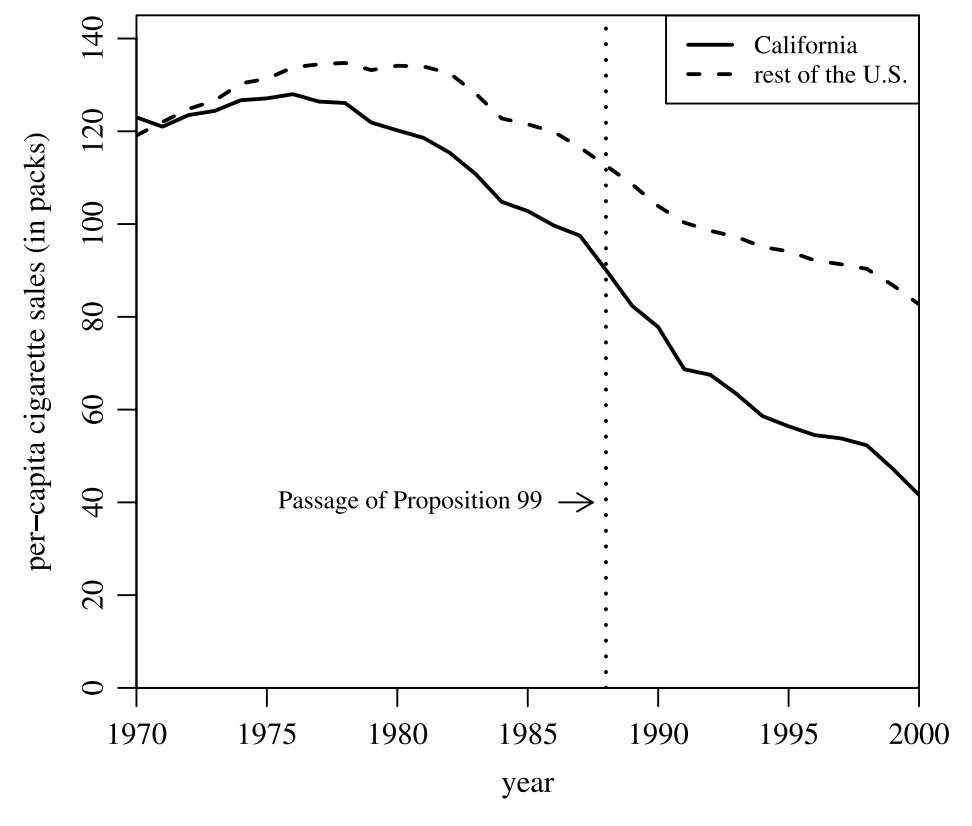
\includegraphics[width = \linewidth]{figures/ca_row.png}
        \end{subfigure} 
        \begin{subfigure}{.45 \textwidth}
            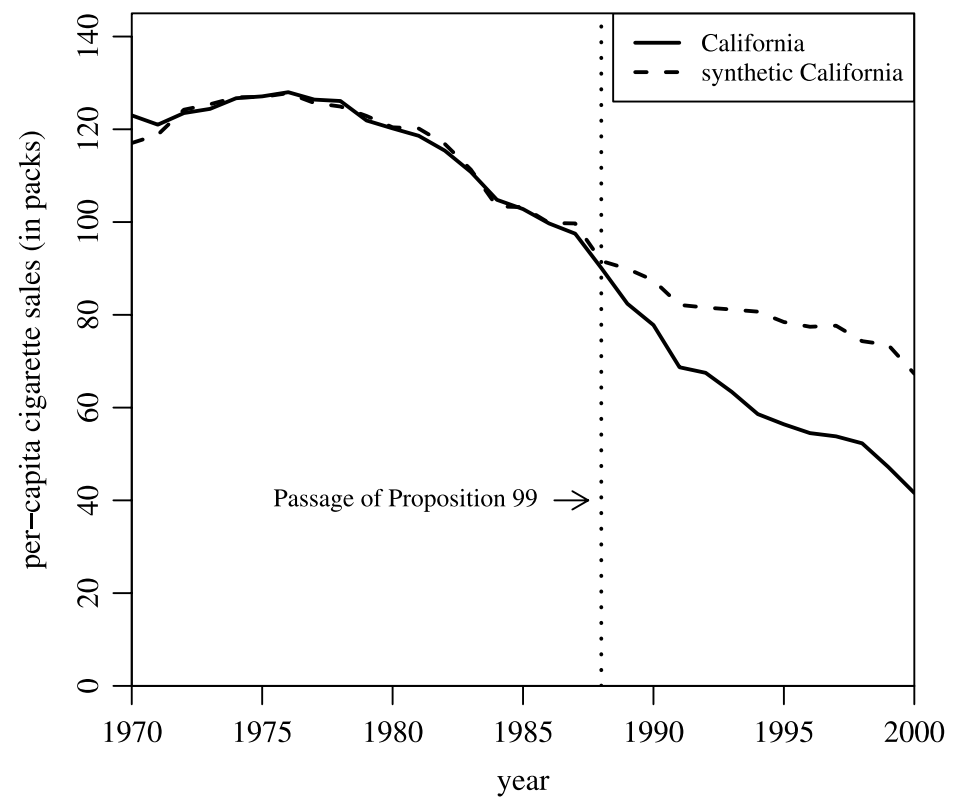
\includegraphics[width = \linewidth]{figures/ca_synthca.png}
        \end{subfigure}
    \end{figure}
    
    Headline: CA cigarette sales p.c. were \textbf{26 packs lower} because of Proposition 99. 
    
\end{frame}

\begin{frame}{}

    Placebo studies are used to quantify the significance of the effect.\pause 
    
    \medskip

    Statistical inferences can be argued via randomization inference framework, and robustness can
    be strengthened by ``in-time placebos."
    
\end{frame}

\begin{frame}{}

    First, a useful construct is the \textbf{mean square prediction error} (MSPE) for unit $i$. \pause 

    \medskip

    Suppose there are $N_c$ control periods and $N$ periods total. Let
    $\hat Y_{it}$ denote the synthetic control for unit $i$ at
    time $t$. Then MSPE over the pretreatment
    period is given by
    $$
    \eta _{\text{pre}} := N_c^{-1}\sum _{t = 1} ^ {N_c} (Y_{it} - \hat Y_{it})^2,
    $$
    and the MSPE over the treatment period is given by
    $$
    \eta _{\text{post}} := (N-N_c)^{-1} \sum _{t=N_c + 1} ^ N (Y_{it} - \hat Y_{it}) ^2.
    $$
    
\end{frame}

\begin{frame}
    Some of the synthetic controls perform quite poorly in the pretreatment period.
    \begin{figure}
        \centering
        \begin{minipage}{0.45\linewidth}
            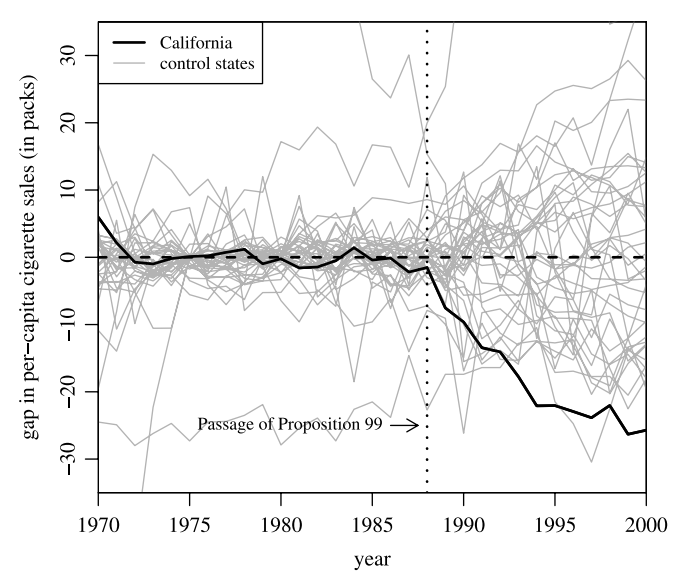
\includegraphics[width=\linewidth]{figures/38donors.png}
        \captionsetup{font=tiny} % Adjust the font size of the caption title
        \end{minipage}
        \caption*{\tiny Time series showing the gap in per-capita cigarette sales using a synthetic control method. The black
        line shows the series for California and the grey lines show the result for all 38 other donor states. States were
        excluded if they enacted large-scale smoking reforms or big taxes between 1989 and 2000.}    \end{figure}
\end{frame}

\begin{frame}
    After subsetting to well performing MSPE in the preintervention period we see a clearer picture.
    \begin{figure}
        \centering
        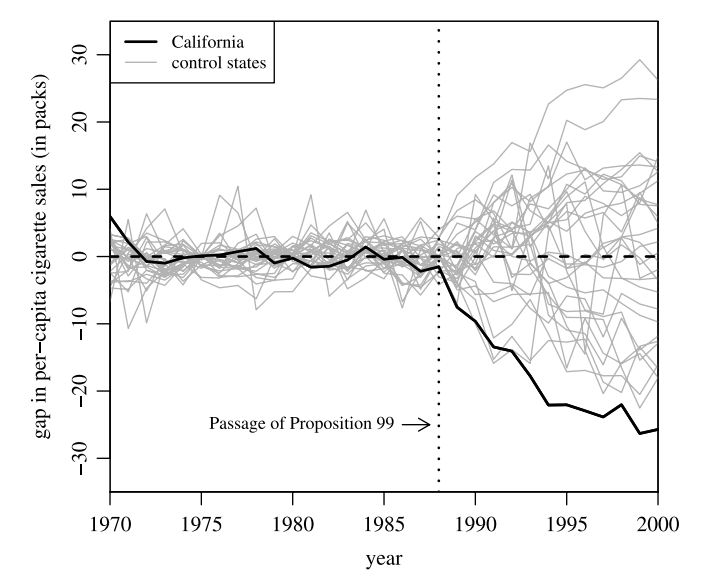
\includegraphics[width = .5\linewidth]{figures/29donors.png}
        \captionsetup{font = tiny}
        \caption*{\tiny Time series showing the gap in per-capita cigarette sales using a synthetic control method. The black
        line shows the series for California and the grey lines show the result for 29 donor states. States were
        excluded if they enacted large-scale smoking reforms or big taxes between 1989 and 2000 or if the mean square prediction error
        greater than five times that of California.}    
        \end{figure}
\end{frame}

\begin{frame}{}
    \medskip 
    Another way to compare synthetic controls is based on the ratio of their posttreatment
    MSPE to their pretreatment MSPE: $\eta _{\text{post}} / \eta _{\text{pre}}$.
    \pause 

    \begin{figure}
        \centering
        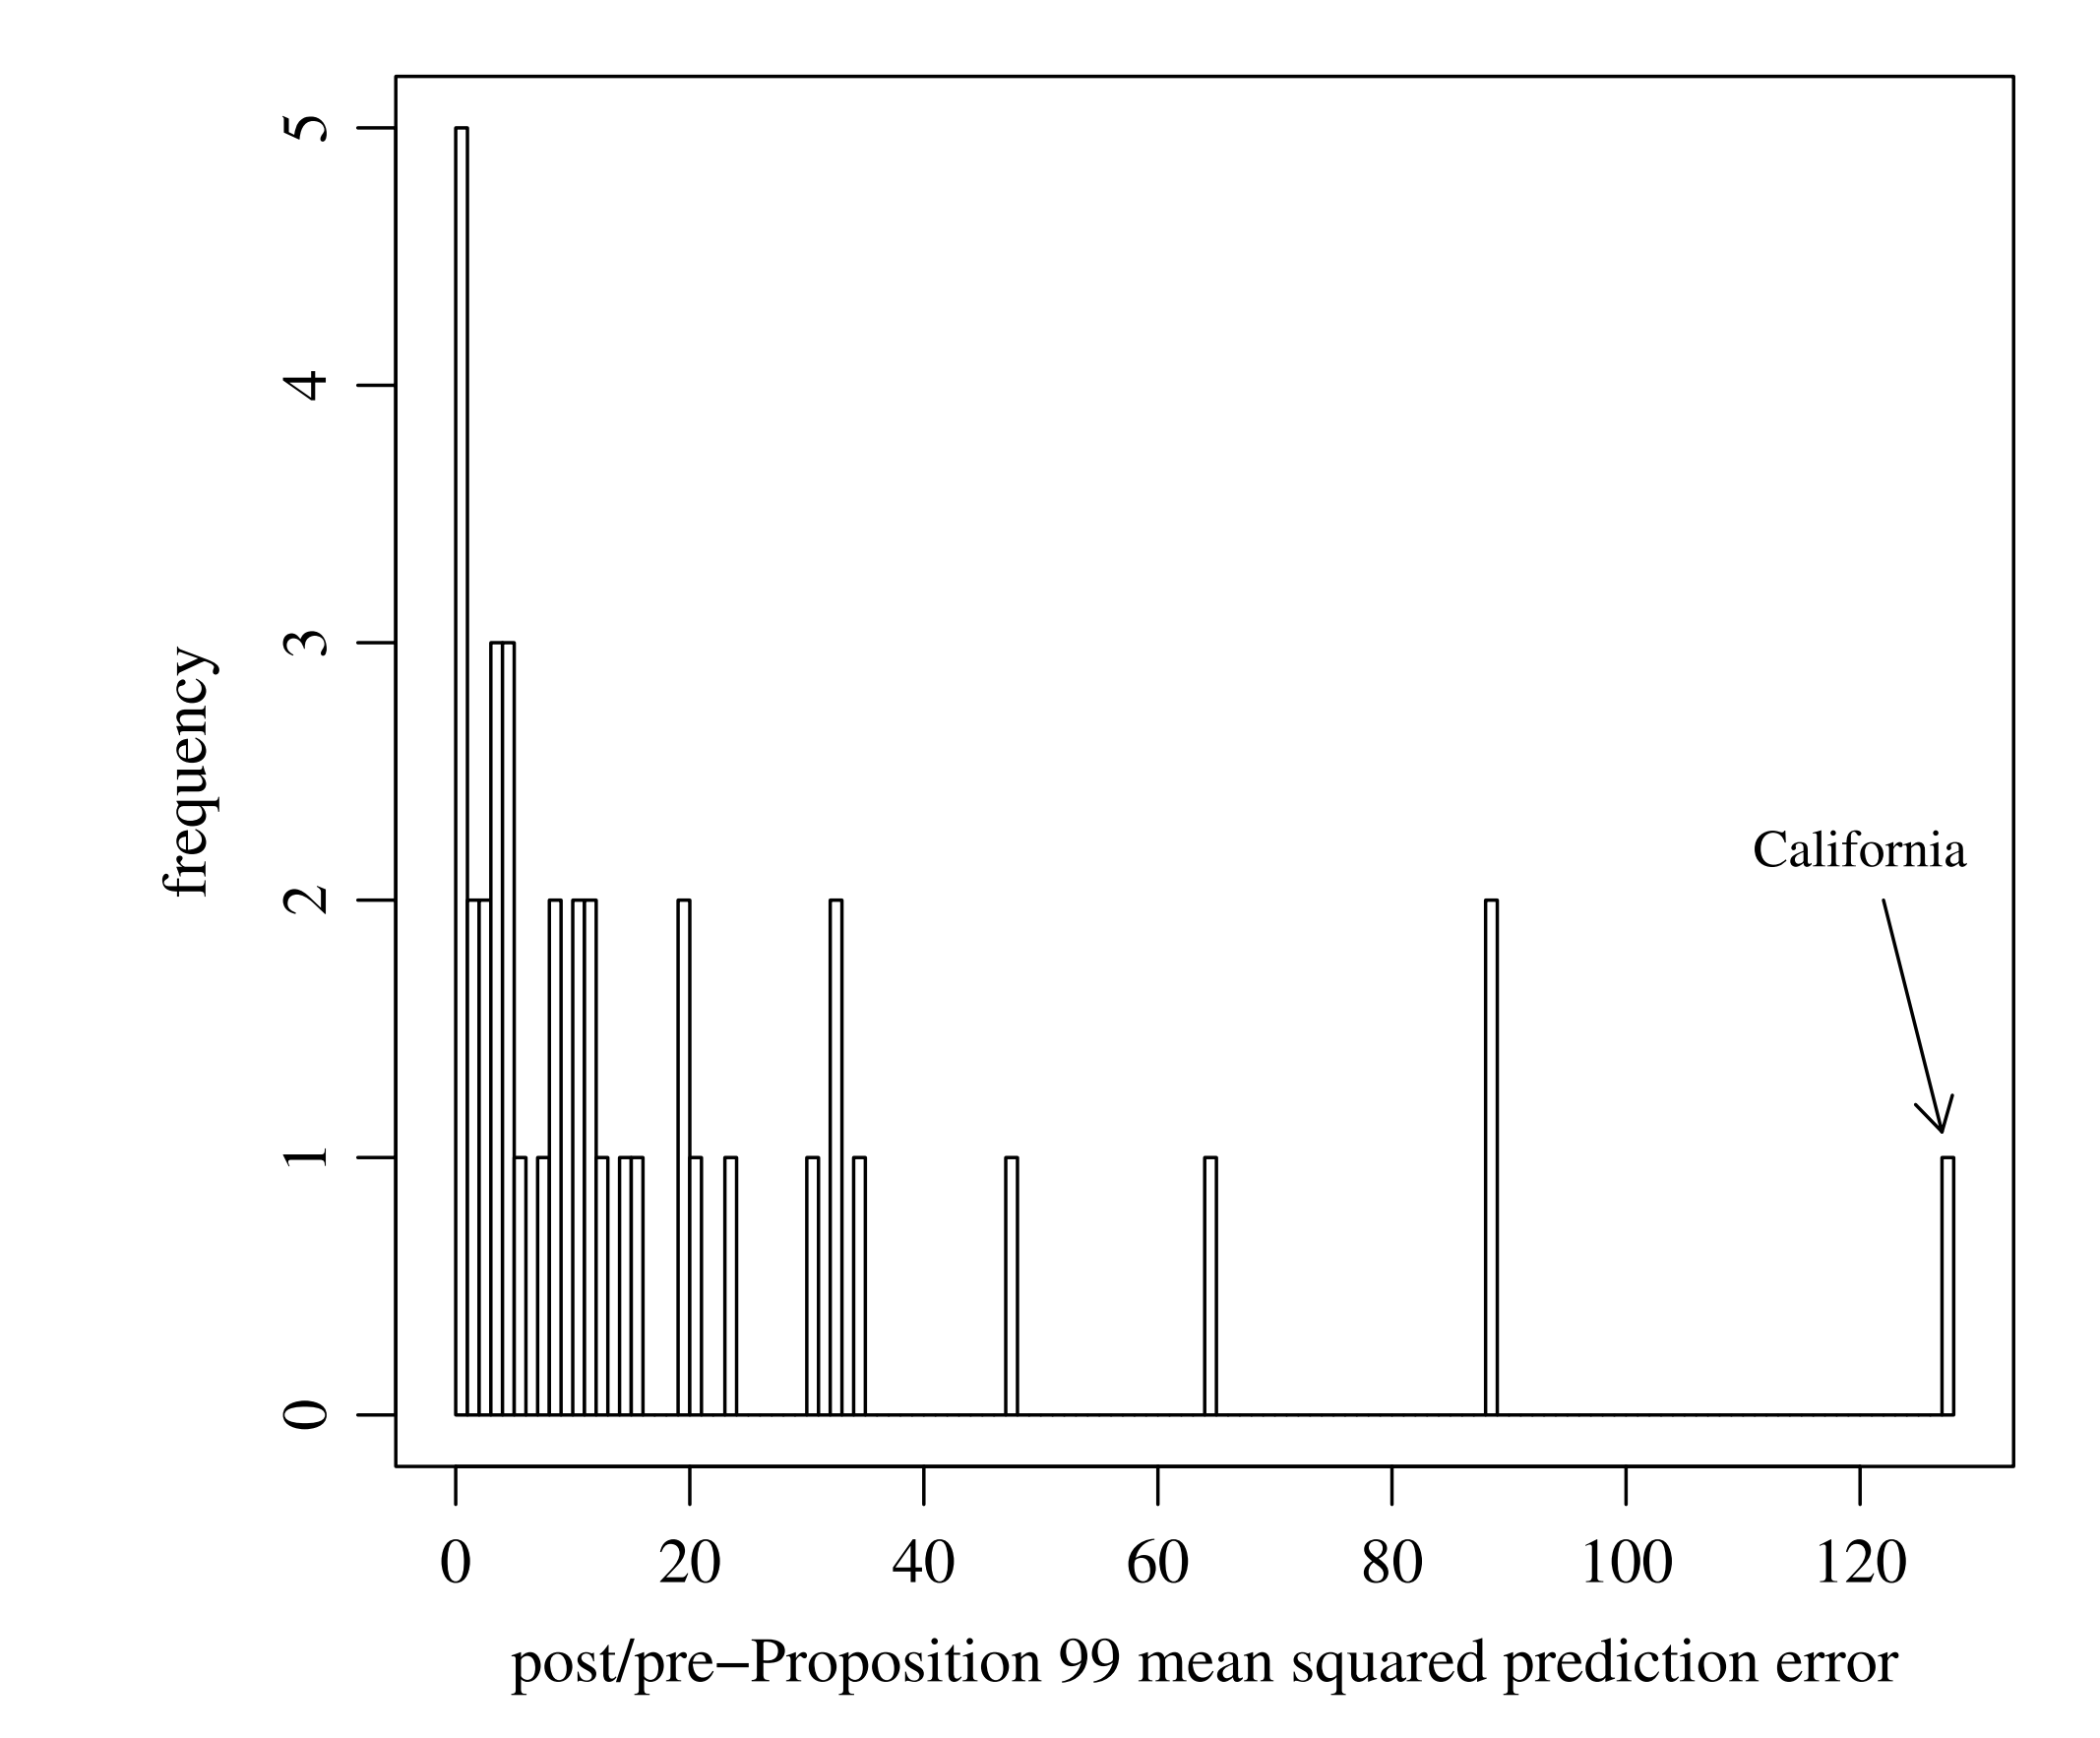
\includegraphics[width = .5\linewidth]{figures/ratio.png}
        \captionsetup{font = tiny}
        \caption*{\tiny A bar chart where the frequency is tabulated over all ratios of posttreatment to pretreatment MSPE. Notice that California stands out drastically in this figure due to the fact that the pretreatment fit is tight, whereas the posttreatment series diverges from the synthetic control.}
    \end{figure}
    
\end{frame}

\begin{frame}{}

    A further diagnostic is to report the results of creating a synthetic control using a different time period of treatment.

    \medskip

    Such a diagnostic is considered an ``in-time" placebo test, in contrast to an ``in-place placebo." \pause

    \medskip
    
    The in-place placebo is introduced in \cite{abadie_comparative_2015}.

\end{frame}


\begin{frame}{}
    \begin{figure}
        \centering
        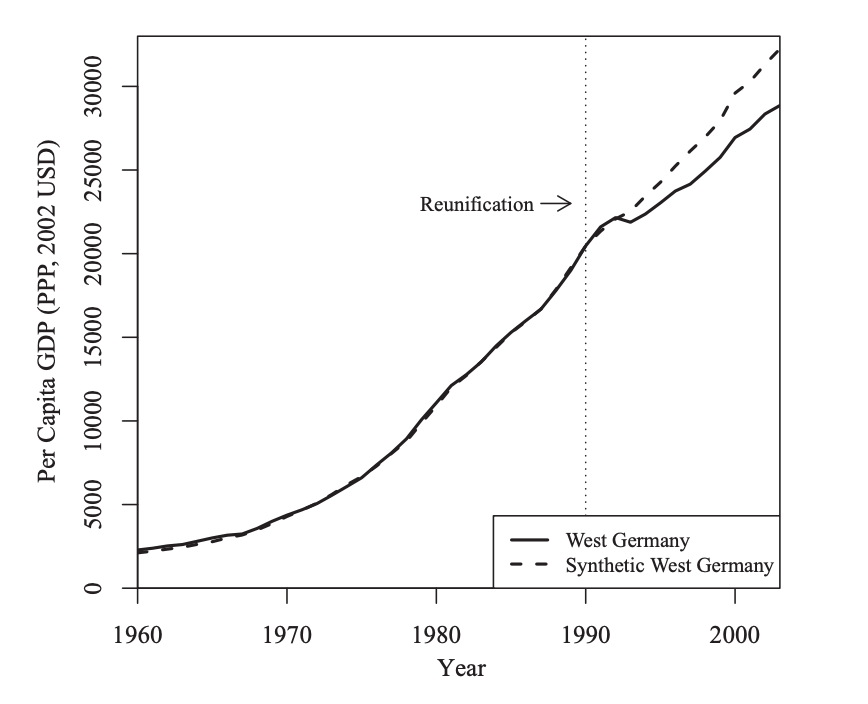
\includegraphics[width = .5\linewidth]{figures/reunif_normal.png}
        \caption*{\small Time series for the evolution of West Germany and a Synthetic Control.
        Source: \cite{abadie_comparative_2015}.}
    \end{figure}
\end{frame}

\begin{frame}{}
    \begin{figure}
        \centering
        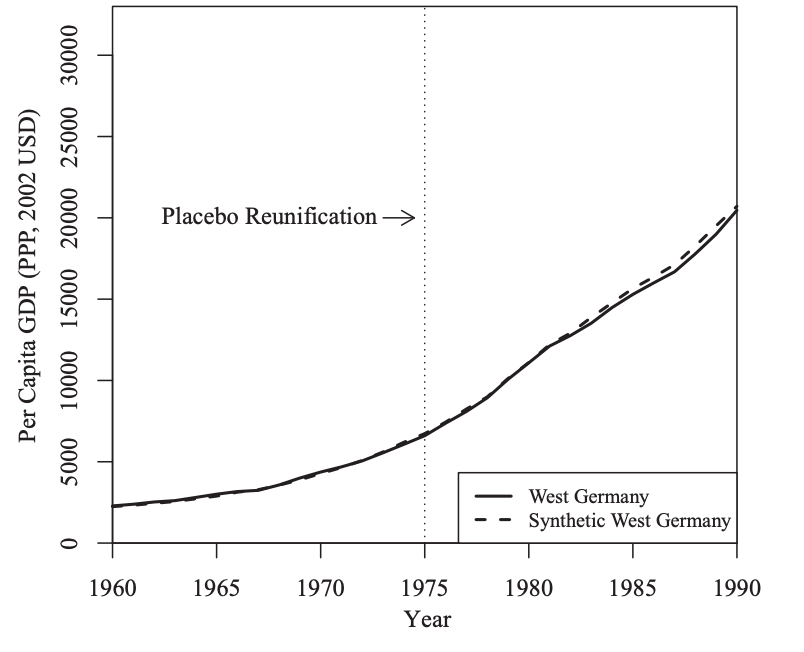
\includegraphics[width = .5\linewidth]{figures/reunif_plac.png}
        \caption*{\small Time series for the evolution of West Germany and a Synthetic Control.
        The synthetic control is an in-time placebo where the year 1975 is taken to be the
        year of the intervention.
        Source: \cite{abadie_comparative_2015}.}
    \end{figure}
\end{frame}

\section{Extensions and conclusion}

\begin{frame}{Extensions}

    \begin{wideitemize}
        \item Regression estimators for case studies also weight observations but might extrapolate
        outside of the convex hull of the data. Synthetic control corrects for this deficiency (\cite{abadie_comparative_2015}).
    
        \item Diff-in-diff is nested in a broader synthetic control
            framework. We simply require that observations receive equal weight in DID (\cite{arkhangelsky_synthetic_2021}).
    
        \item Cross-validation and jackknife techniques for variance estimation that fall outside of the
        basic randomization inference setting that we have discussed.        
    \end{wideitemize}
    
\end{frame}

\begin{frame}{Conclusion}
    \begin{itemize}
        \item Synthetic control is an influential technique for causal inference despite its relative novelty.
        \item Theory provides justification for statistical statements about the estimated treatment effects.
        \item Empirical applications abound in settings where the number of treated is relatively small.
        \item Research in both applied and theoretical settings is active and ongoing.
    \end{itemize}

\end{frame}

% BIBLIOGRAPHY
\begin{frame}[allowframebreaks]{References}
\printbibliography
\end{frame}

\end{document}